\documentclass[a4paper,fleqn]{cas-dc}

%\usepackage[authoryear,longnamesfirst]{natbib}
\usepackage[authoryear]{natbib}
%\usepackage[numbers]{natbib}

% Quotes
\usepackage{csquotes}

% Colors
%\usepackage[usenames]{color}

% Let us have multiline comments
\usepackage{verbatim}

% Footnotes in section headings
%\usepackage[stable]{footmisc}

% Mathematics, Code and tables
\usepackage{amsmath}
%\usepackage{bm}
%\usepackage{amsfonts}
\usepackage[group-separator={,}]{siunitx}
\usepackage{xfrac}
%\usepackage{mathtools}
\usepackage{alltt}
\usepackage{algorithm}
\usepackage{algpseudocode}
\usepackage{multirow}

\usepackage{listings}
\lstset{
    basicstyle=\ttfamily
}

% Have graphics
\graphicspath{{images/manual/}{images/computed/}}
\usepackage{subfig}
\usepackage{caption}
\captionsetup[subfloat]{margin=0.5em}

% Be smart with ref names
\usepackage{cleveref}

% Help in placing the floats
\usepackage{placeins}

% Have numbered quotes
\setlength{\leftmargini}{3em}
\newsavebox\nquotebox
\newenvironment{nquote}
  {\begin{equation}
   \begin{lrbox}{\nquotebox}
   \begin{minipage}{\dimexpr\columnwidth-2\leftmargini}
   \setlength{\leftmargini}{0pt}%
   \begin{quote}}
  {\end{quote}
   \end{minipage}
   \end{lrbox}\makebox[0pt]{\usebox{\nquotebox}}
   \end{equation}}

% To make comments, corrections, notes
\newcommand{\tb}[1]{\textcolor{blue}{#1}}
\newcommand{\rk}[1]{\tb{{\footnotesize {\bf[\emph{#1}]}}}}
\newcommand{\marginnote}[1]{\marginpar{{\parbox{1.\linewidth}{\hrulefill\\\tb{\scriptsize \sf #1}}}}}
\newcommand{\cam}[1]{\tb{\small{[{\bf C:} }#1{]}}}
\newcommand{\seb}[1]{\tb{\small{[{\bf S:} #1{]}}}}

% If citations or references are missing, make it visible
\newcommand{\CN}{\textsuperscript{\tb{[Citation needed]}}}
\newcommand{\CNs}{\textsuperscript{\tb{[Multiple citations needed]}}}


\begin{document}
%\let\WriteBookmarks\relax
%\def\floatpagepagefraction{1}
\def\textpagefraction{.001}
%% TODO: define a proper short title
\shorttitle{Gistr}
%\shortauthors{}

\title[mode=title]{Transformations in large-scale text transmission chains}

\author[1]{Sébastien Lerique}[orcid=0000-0002-5787-8397]
\cormark[1]
\ead{sebastien.lerique@normalesup.org}
\ead[url]{slvh.fr}
\credit{TODO: credits}
\address[1]{Embodied Cognitive Science Unit, Okinawa Institute of Science and Technology Graduate University, Onna-son, Okinawa 904-0495, Japan}

% TODO[cam]: add orcid id
\author[2,3]{Camille Roth}
\ead{roth@cmb.hu-berlin.de}
\ead[URL]{camilleroth.eu}
\credit{TODO: credits}
\address[2]{Camille's first affiliation}
\address[3]{Camille's second affiliation}

\cortext[cor1]{Corresponding author}

\begin{abstract}
  \rk{TODO: abstract}
\end{abstract}

%% TODO: graphical abstract
%% \begin{graphicalabstract}
%% \includegraphics{figs/grabs.pdf}
%% \end{graphicalabstract}

%% TODO: highlights
%% \begin{highlights}
%% \item Research highlights item 1
%% \item Research highlights item 2
%% \item Research highlights item 3
%% \end{highlights}

\begin{keywords}
  TODO: keywords \sep more keywords
\end{keywords}

\maketitle


%% -----------------------------------------------------------------------------------------------------------------------------------------


\section{Introduction}\label{sec:gistr-intro}

The previous chapter demonstrated that it is possible to observe
cognitive biases in the way quotations are copied from blog to blog. By
grounding those biases in known effects in the recall of word lists, we
also showed that the enquiry of cultural evolution for linguistic
content can be related to lower-level cognitive mechanisms that help
understand the way content is transformed in ecological situations.
However in the online corpus we considered only extremely simple
transformations, namely individual word replacements, so as to be able
to infer missing links between quotations and thus make the analysis
possible. While we observed a reliable bias in the way words are
replaced, consistent with known psycholinguistic biases, our view of the
overall transformations is extremely narrow: not only is it restricted
to word replacements, it is limited to the replacements that were the
only change in an utterance (other than sentence cropping). The analysis
also remained at the low-level of lexical properties such as word
frequency and age of acquisition, neither of which give much insight
into the semantic changes that utterances can undergo. Finally,
constraints of the data did not let us identify chains of
transformations, and we could not observe the evolution of quotations
beyond the individual transformation step.

We now wish to remedy most of these points by studying the evolution of
short utterances in a controlled experimental setting. A controlled
setting means having a less ecological situation, but also allows for
the collection of all the available data for analysis. Once again, our
approach is exploratory, and we aim to reach a more complete
understanding of the transformation process that is at work in the
propagation of online quotations, but also more widely in the evolution
of written utterances as they are transmitted using other mediums. Our
reasoning is that by better understanding the transformations undergone
by such utterances, we will gain insight into the way actual linguistic
representations may change because of interpretation and memory
mechanisms.

More precisely, our goal is to construct a descriptive model of the
process that can bring insight into why utterances change the way they
do, and how such observations can be connected to current knowledge in
linguistics, on one side, and to the broader cultural evolution
frameworks, on the other. Indeed, current knowledge of the
transformation of utterances is quite partial: laboratory transmission
chains show that a number of high-level biases appear in the
transmission of purposefully constructed complex stories, but do not
explain in detail how such trends come about. On the other hand, the
psycholinguistics literature on sentence recall shows that there are
important semantic and syntactic effects in the way sentences are
reformulated, but they do so on extremely simple types of content that
make it difficult to generalise results. There seems to be a missing
link between the high-level effects observed in
transmission chains of complex stories and the lower-level processes known to act in the recall of simple sentences. A descriptive
model of transformations would go a long way in creating this link, and would thus help to explain more easily the overall evolution of utterances in terms of lower-level cognitive mechanisms.

One of the ideal setups to tackle this question would be a standard transmission
chain where we observe the accumulated transformations made by
participants on a set of utterances that we choose.
%However, given our exploratory approach and the fact that we do not know in advance what the model will look like, it is important that we can run several such experiments in short cycles so as to adjust the task parameters and the sampling of utterances. It is also important that the collected data be of similar size to the number of substitutions we extracted in the previous chapter, so that we will be able to compare and validate any overlapping results.
We therefore decided to run a set of transmission chain experiments on an online platform developed for the purpose: as we shall see, after an initial development phase this approach lets us collect large amounts of data in short periods of time, while maintaining a level of control similar to that of laboratory experiments.

We begin by discussing the works relevant to this endeavour, and in
particular the bind in which current transmission chain experiments on
linguistic content find themselves. We then present the procedure
followed to develop the online experimental platform, and the measures
implemented to achieve a high level of quality in the data. Next, we
expose our analysis of the data sets collected, present the descriptive
model of transformations we construct from them, and highlight the main
behaviours the model lets us observe. Finally, we discuss the relevance
of these results in the broader context of the study of cultural
evolution.

\section{Related work}\label{sec:gistr-related}

Inspired by the selectionist models of culture developed by
\citet{boyd_culture_1985} and
\citet{cavalli-sforza_cultural_1981}, a sizeable part of the
empirical work on cultural change has focused on identifying and separating content and
context biases in the way cultural items are transmitted. This line of
work relies heavily on the transmission chain paradigm initially
introduced by \citet{bartlett_remembering:_1995}. For linguistic
content in particular, studies using that paradigm now provide a
catalogue of contrasts in the way utterances or short stories are
transmitted. These effects range from the stereotypical personification
of objects \citep{bangerter_transformation_2000}, the favouring of
negative story aspects \citep{bebbington_sky_2017} or the increased
hierarchical encoding of events \citep{mesoudi_hierarchical_2004}, to
biases in favour of social \citep{mesoudi_bias_2006} or
counter-intuitive aspects of stories
\citep{norenzayan_memory_2006,barrett_spreading_2001}. Other
effects such as the role of emotions in the selection of items to
reproduce \citep{heath_emotional_2001,eriksson_corpses_2014}, or
conformity and prestige biases \citep{acerbi_did_2017} have been
studied by focusing on the individual transmission step on which the
evolution of content hinges.

Often, such effects are identified by selecting two or more minimally
different types of content and contrasting the way they evolve in
transmission chains (for instance measuring the rate at which they are
degraded). When a type of content is significantly better transmitted
than other types, it signals that a bias is acting on that contrast
dimension. The technique is useful in the context of selectionist models
of culture, as it identifies examples of biases which could create
selection pressures for specific cultural types and thus drive cultural
evolution. It is also relevant to the Cultural Attraction framework,
which focuses on the aspects of culture for which reconstructive
processes are more important than selection. For instance, the approach
recently introduced by \citet{claidiere_how_2014} proposes to
use evolutionary causal matrices to model such attraction-based
processes in cultural evolution, and could gain insight from the trends
observed in transmission chains.
%In the terminology of
%\citet{morin_how_2016}, selectionist models focus on how culture
%survives in spite of wear-and-tear, and cultural attraction focuses on
%how culture survives in spite of possible flops, where a given item
%fails to elicit sufficient interest to be recreated at all.
In theory,
both selection and attraction can be observed in transmission chains. However, in
its current implementation focused on contrasting outcomes between
several (usually two) conditions, the technique gives little insight
into the underlying mechanisms at work, and into how exactly such processes
can be described and explained in terms of cognitive %and situated
processing.

Indeed, understanding the mechanisms behind transformations in chains, or even only quantitatively describing the details of said transformations, remains very much a challenge.  This is especially true in the linguistic domain where the complexity of language hinders most attempts to comprehend sentence evolution. Now the current literature features two typical strategies to study such transformations. The first one trivially consists in doing the analysis by hand.  Here, we may further distinguish approaches relying on in vitro content, where data is produced by ad hoc experiments whose participants are asked to reformulate content under certain conditions, from approaches using in vivo content, usually based on large text datasets.
For instance, the study of the propagation of risk perception developed by \citet{moussaid_amplification_2015} used an interaction setting where subjects were filmed while freely discussing a topic. The recorded conversations were later hand-coded for the presence of certain information items introduced at the beginning of the chains. On the in vivo side, \citet{lauf_analyzing_2013} carried out a linguistic analysis of transformations of quotes in a corpus of news stories by exhaustively hand-coding differences between sentences.

The second strategy consists in using automated methods.  In the in vivo case, this generally requires to focus on a tightly constrained type of transformation, and possibly rely on some empirical proxies, as there is no control over the conditions of production of the observed sentences. %It also relies on pre-labelled data sets, often from online platforms, on which machine learning techniques can extract features that correlate to the transmission of pieces of content.
For instance, our recent analysis of single word substitutions in quotations observed in a large blog post dataset \citep{lerique-2018-semantic-drift} belongs to this category.
In a slightly different setting, \citet{danescu-niculescu-mizil_you_2012} study the memorability of movie quotes by exploiting user ratings provided on the Internet Movie Database website. While their study does not focus on the transformation of content per se, it illustrates the types of memory-related features that may also help explain transformations.

In an in vitro setting, linguistic content evolution is found in the study of intrusions in the recall of word lists \citep[see][for a review]{zaromb_temporal_2006}, and in the study of word replacements and simple syntactic changes in short sentences \citep{potter_regeneration_1990,lombardi_regeneration_1992}.
%the observation of linguistic content evolution can be found in the study of intrusions in the recall of word lists \citep[see][for a review]{zaromb_temporal_2006}, and in the study of word replacements and simple syntactic changes in short sentences \citep{potter_regeneration_1990,lombardi_regeneration_1992}.
These are much simpler transformations than transformations of complete sentences, and are thus more amenable to statistical analysis. Note that a similar focus on lower-dimensional changes is found in non-linguistic studies, such as iterated learning on sequences of colour items for which standard regularity metrics exist \citep{cornish_systems_2013}, or transmission chains of constrained visual patterns such as those used by \citet{claidiere_cultural_2014}. Both cases feature discrete and combinatorial pieces of content, for which it is possible to use standard notions of distance, equality, or regularity in transformation.



%In an in vitro setting, the only type of observed linguistic content evolution relies on single words –-- either in the case of the study of intrusions in the recall of word lists \citep[see][for a review]{zaromb_temporal_2006}, and that of word replacements in short sentences \citep{potter_regeneration_1990,lombardi_regeneration_1992}
%%These studies can be seen as employing that strategy:
%--- word intrusions in lists and individual replacements in sentences
%both processes are much simpler than transformations of complete sentences, and are thus more amenable to statistical analysis. To the best of our knowledge, no experimental study has so far described sophisticated transformations at the sentence level in an automated manner.
%%In other words, automated analysis of in vitro content tightly constrains the linguistic features, for instance sentences of a very specific type, or for which only pre-defined changes can happen. %In that case the transformations can be directly modelled to identify regularities.



%%Indeed, understanding the mechanisms behind transformations in chains,
%%or even only quantitatively describing the details of said
%%transformations, remains very much a challenge. This is especially true
%%in the linguistic domain, where the complexity of language hinders most
%%attempts to understand what is going on in a transformation. Up to now
%%three main strategies have been developed to delve into to detail of
%%transformations. The first is to use tightly constrained linguistic
%%content, for instance sentences of a very specific type, or for which
%%only pre-defined changes can happen. In that case the transformations
%%can be directly modelled to identify regularities. The study of
%%intrusions in the recall of word lists \citep[see][for a
%%review]{zaromb_temporal_2006}, and that of word replacements in short
%%sentences
%%\citep{potter_regeneration_1990,lombardi_regeneration_1992}, can be
%%seen as employing that strategy: word intrusions in lists and individual
%%replacements in sentences are much simpler than transformations of
%%complete sentences, and are thus more amenable to statistical analysis.
%%Our analysis of single word substitutions in quotations observe in a large blog post dataset \citep{lerique-2018-semantic-drift} can be categorised here too. A similar strategy is found in non-linguistic
%%studies, such as iterated learning on sequences of colour items for
%%which standard regularity metrics exist \citep{cornish_systems_2013},
%%or transmission chains of constrained visual patterns such as those used
%%by \citet{claidiere_cultural_2014}. Both cases feature discrete and
%%combinatorial pieces of content, for which it is possible to use natural
%%notions of distance, equality, or regularity in transformation. This
%%first strategy can be termed the \enquote{simple setting} strategy.
%%
%%At the other end of the spectrum we find the \enquote{do-it-by-hand}
%%strategy. This approach uses more ecological content but relies on
%%exhaustively hand-coding it, and is used in most of the transmission
%%chain studies mentioned above. The study of risk perception propagation
%%developed by \citet{moussaid_amplification_2015}, for instance, used
%%a free-form interaction setting where subjects were taped while freely
%%discussing a topic. The recorded conversations were later hand-coded for
%%the presence of certain information items introduced at the beginning of
%%the chains. The linguistic analysis of transformations of quotes in news
%%stories provided by \citet{lauf_analyzing_2013} is also the product
%%of exhaustively hand-coding differences between sentences.
%%
%%Finally, the third strategy relies on pre-labelled data sets, often from
%%online platforms, on which machine learning techniques can extract
%%features that correlate to the transmission of pieces of content. This
%%is the \enquote{already coded} strategy.
%%\citet{danescu-niculescu-mizil_you_2012}, for instance, study the
%%memorability of movie quotes by exploiting user ratings provided on the
%%Internet Movie Database website. While their study does not focus on the
%%transformation of content per se, it illustrates the types of
%%memory-related features that pre-labelled data sets can help extract in
%%order to explain transformations. Conversely, analysing the regularities
%%that arise in unlabelled digital traces often falls back into the first
%%strategy: without an outsourced coding of the data, analysing
%%unconstrained real-life interactions is so complex that one often has to
%%focus on a limited set of features in the available data, thus proposing
%%a \enquote{simple setting} analysis. As we saw in the previous chapter,
%%the analysis of partial digital traces can also fall back into the first
%%strategy, as having to infer missing information led to drastically
%%simplifying the transformations considered.
%%
%%Strategies two and three are additionally closely tied to data
%%collection methods. Free-form interaction and more generally ecological
%%content is costly to hand-code, and thus necessarily limited in size; it
%%is also best used in controlled settings where the choice of content can
%%be optimised. Conversely, using machine learning to extract features
%%that relate to content transmission requires large amounts of
%%pre-labelled data, which often means that an existing public data set
%%must be used. Such studies thus seldom control the conditions under
%%which the data is generated, which restricts the interactions they can
%%explore to those encoded in existing data sets: any behaviour or piece
%%of content that is not observable in public data sets is off limits.

%%Overall, studies targeted at understanding the details of
%%transformations of linguistic content seem forced to pick two of the
%%following three properties, and relinquish the third: realistic content,
%%computational analysis, and control over the generation of the data.
%%Picking \enquote{realistic content and computational analysis} leads to
%%the \enquote{already coded} strategy. Picking \enquote{realistic content
%%and control over data generation} requires hand-coding a substantial
%%part of the data collected, that is strategy two. Finally,
%%\enquote{computational analysis and data generation control} leads to
%%the \enquote{simple setting} strategy. This bind thus appears as a major
%%challenge to the better understanding of changes in linguistic content,
%%and more broadly to the study of language-related cultural evolution. In
%%particular, it hinders attempts to model the low-level processes which
%%could provide a more parsimonious account of the contrasts observed in
%%linguistic transmission chains, and allow for a deeper integration of
%%the study of cultural evolution with linguistics.

To the best of our knowledge, no experimental study so far has described sophisticated transformations at the sentence level in an automated manner.
To overcome this obstacle we turn to two related fields of research. The
first, which we term the Web and Smartphone experimental approach, %is creating a middle ground between controlled laboratory experiments and the analysis of online corpora. This approach
takes advantage of the ubiquity of internet browsers and mobile computing to develop
large-scale controlled experiments out of the laboratory.
\citet{miller_smartphone_2012} %discusses the possibilities opened by developing experiments as smartphone applications in particular, and
notes that this method changes the logistics %and context-awareness
of experiments: large amounts of subjects can be recruited online without
having to manage meeting schedules, %, and experiments can probe
%participants without interrupting their everyday life, both
an advantage
that has been exploited in the study of mind-wandering and happiness
\citep{killingsworth_wandering_2010,mackerron_happiness_2013,bastian_language_2017},
%A closely related method is the development of experiments as web
%applications, which similarly changes the set of experimental
%constraints.
%In linguistics, the possibility for large-scale data
%collection has been successfully used in
 vocabulary size
\citep{keuleers_word_2015,brysbaert_how_2016}, %; creating studies
%that involve many subjects at the same time is also made much simpler by
%the online logistics, an advantage that has been used for instance in
%the study of
or group conversations \citep[][which also involves many subjects simultaneously]{niculae_conversational_2016}.
%More generally, these approaches relax the opposition between
%small-scale controlled experiments in the laboratory on one side, and
%analyses of large-scale but passively collected online data on the other
%side.
Once the initial development cost is covered, this approach makes it
possible to collect relatively large data sets in short cycles, and
combines simplified logistics with a level of control similar to that of
laboratory experiments.

The second field we rely on creates an opening for the detailed
modelling of utterance transformations: biological sequence alignment,
the sub-field of bioinformatics which seeks to uncover commonalities in
sequences of DNA, RNA, or amino acids in proteins from different
species, has developed over the last 50 years a range of general
algorithms to relate sequences of items. One such algorithm in
particular, introduced by \citet{needleman_general_1970}, extends the
principles of the Levenshtein distance and is particularly well suited
to the analysis of linguistic transformations when combined with
standard natural language processing methods. Inspired by
\citet{lauf_analyzing_2013} who use similar tools to prepare their
data for manual analysis, we use and extend the Needleman-Wunsch
algorithm to reliably extract regularities in the way utterances are
transformed through transmission chains.


%% -----------------------------------------------------------------------------------------------------------------------------------------


\section{Methods}\label{sec:gistr-methods}

\subsection{Experiment design
principles}\label{experiment-design-principles}

\subsubsection{Advantages and challenges of transmission
chains}\label{advantages-and-challenges-of-transmission-chains}

An obvious way to address the questions raised in the previous chapter
is to use transmission chains in the laboratory to study the evolution
of online quotations in a controlled setting: each subject reads,
retains, and rewrites sentences that are then passed on to the next
subject in a chain of reformulations. Such a setup can reproduce an
idealised version of the read-remember-rewrite process which, we
hypothesised, participates in the evolution of quotations in blogspace
and media outlets. It also provides the information that our previous
data set lacked in order to analyse the complete transformations of
quotations, as well as the long-term effect of those changes: the links
between parent and child sentences are naturally encoded in the data,
such that the transformations undergone by each sentence can be studied
in full detail. There is no need to restrict ourselves to simpler
changes as was necessary for the inference procedure used with digital
traces from blogspace. By creating an artificial setting, the experiment
design also lets us control the reading and writing conditions as well
as the context in which sentences appear, which further removes one of
the inevitable uncertainties of the previous protocol (albeit at the
cost of less ecological conditions).

However, the laboratory transmission chain paradigm is not a good fit
for our exploratory approach: we aim to collect data that will allow us
to study both the complete set of transformations undergone by short
utterances such as online quotations, and the interactions and
cumulative effect of such changes; yet we do not know in advance the
types of changes that subjects will make, or the extent to which such
changes vary according to the type of linguistic content. Transmission
chain studies typically start with an a priori hypothesis focused on a
well-identified type of content, which is then empirically tested by
contrasting the evolutionary outcome of two classes of sentences.
Instead, our goal here is to provide first steps to characterise the
process by which such evolution of linguistic content arises, and
observe how it accumulates in the long term. The setup must thus allow
us to collect enough data to extract regularities in successive
transformations operated by different subjects on different sentences,
and provide a resolving power similar to that of substitutions in online
quotations so that we can compare results with the previous chapter.
Since our main target is the set of detailed transformations and their
interactions, a phenomenon of higher dimensionality than the contrast of
accumulated outcomes, it is also crucial to fine-tune the difficulty of
the read-write task and the complexity of the source sentences, in order
to trigger a set of transformations varied enough that it could approach
some of the changes encountered in real life situations. Our progress
therefore involves a non-trivial trial-and-error component: indeed, a
task made too easy or too difficult, and more so a set of source
sentences that are too complex or too straightforward, will lead to
either mass deletions or perfect conservation (or the former followed by
the latter), none of which can help characterise the more intricate
changes that linguistic content undergoes in the ecological setting we
aim to simulate.

%%\subsubsection{Web and smartphone experiments}\label{web-and-smartphone-experiments}
%%
%%Complementary to laboratory studies and to approaches using online
%%digital traces, a new empirical approach based on Web browsers and
%%mobile computing is striking a different balance in the trade-offs of
%%experimental work; it seems very promising in addressing the problems
%%outlined above. Indeed, browsers (both on desktop and mobile) and
%%smartphones have evolved into powerful, ubiquitous application
%%environments for which one can develop any kind of experiment involving
%%text, graphics, and human interactions. At the cost of increased
%%engineering requirements and a different approach to subject
%%recruitment, Web and smartphone experiments give the designer full
%%control over what data is collected and the way interactions are framed
%%(similar to laboratory experiments), and make it possible to quickly
%%collect data sets at scales comparable to what filtered and cleaned
%%digital traces provide.
%%
%%This approach makes a number of unusual trade-offs, the benefits of
%%which can be summarised as follows:
%%
%%\begin{itemize}
%%\item
%%  \emph{Control}: similar to laboratory experiments, and unlike digital
%%  trace analysis, it is possible to use complex designs where all the
%%  interactions of the subjects are framed and observed by the
%%  experimenter. This includes for instance the presentation of the
%%  experiment (e.g.~as a game or a self-improvement aid, aside from being
%%  a scientific study) and, more importantly, the ways in which the
%%  system mediates the interactions between the subjects.
%%\item
%%  \emph{Scale}: if and when needed, the technical platform can scale the
%%  number of subjects to the tens of thousands at low marginal cost.
%%  Interactions between subjects can also scale to involve synchronous or
%%  asynchronous contact between hundreds of people, without having to
%%  manage per-subject scheduling.
%%\item
%%  \emph{Speed of data collection}: once the initial development is
%%  completed (see costs below), the data collection cycle is short. One
%%  day can be enough to collect \num{1000}--\num{10000} usable data
%%  points, a size comparable to the final substitutions set extracted and
%%  analysed in the previous chapter. This is especially relevant for
%%  exploratory work which is made much easier with shorter
%%  trial-and-error cycles.
%%\item
%%  \emph{Flexible recruitment}: while also a challenge (see costs below),
%%  subject recruitment is more flexible than in the laboratory: services
%%  like Prolific Academic\footnote{\url{https://www.prolific.ac/}.} let
%%  the experimenter recruit at reasonable costs in pools of tens of
%%  thousands of subjects with fine-grained demographic filters. Wider
%%  audiences can be achieved by offering non-financial rewards, framing
%%  the experiment as a self-improvement application, or turning it into a
%%  game.
%%\end{itemize}
%%
%%The corresponding costs are the following:
%%
%%\begin{itemize}
%%\item
%%  \emph{Technical challenge}: developing Web and smartphone experiments
%%  involves a substantial amount of engineering, and makes use of
%%  technologies that most researchers, even technical, are not familiar
%%  with. While a couple of all-in-one kits exist,\footnote{See e.g.
%%    \url{http://funf.org/} and \url{http://www.epicollect.net/}.}
%%  creating an experiment that meets one's research questions requires
%%  learning average skills in most of the technologies at play: a native
%%  or cross-platform smartphone development environment, Web application
%%  development, backend server programming, and some server
%%  administration skills. Most importantly, the paradigms and problems
%%  encountered are new to researchers: control flow is asynchronous due
%%  to network communication and the user interface, and technicalities
%%  such as user management or email validation can grow into difficult
%%  engineering challenges.
%%\item
%%  \emph{Spam-control}: subjects are not constrained or encouraged by the
%%  face-to-face interaction of a laboratory experiment, neither are they
%%  (in most experiments) in the course of an interaction with friends
%%  that provides natural incentives for what they write, as can be the
%%  case with digital traces. Participants must have an incentive to
%%  perform the experiment's tasks well. If the spam introduced by one
%%  subject can be isolated in the design of the experiment, one
%%  possibility is to filter it after data collection and make payment
%%  depend on its prevalence. But if the spam introduced by one subject
%%  naturally propagates to data seen by other subjects in the experiment,
%%  as is the case for transmission chains, effective anti-spam pressures
%%  and motivations need to be factored into the design.
%%\item
%%  \emph{Recruitment cost}: while recruiting up to a few hundred subjects
%%  is cheaper than the equivalent for a laboratory experiment (not
%%  counting the development cost),\footnote{Global competition on online
%%    platforms like Prolific Academic drives subject payments down.} and
%%  is easy to manage for fast prototyping and pilot tests, recruitment
%%  cost rises linearly with the number of subjects and the time they
%%  spend on the experiment, unless a different strategy is used. Turning
%%  an experiment into a playful application or an application useful to
%%  the subjects (effectively making them users) involves yet another set
%%  of skills, can prove challenging, and must be factored into the
%%  development cost.
%%\end{itemize}

\subsubsection{General setup for Web-based transmission
chains}\label{general-setup-for-web-based-transmission-chains}

The balance achieved by Web-based experiments is well adapted to the
requirements we outlined above. Since no existing system would fit our
needs, we chose to develop a tailored Web-based platform that could run
transmission chains as Web experiments. Once ready, the platform would
allow us to gather sufficient amounts of quality data in short cycles.
We further decided to implement the simplest possible version of the
transmission chain paradigm that is still viable, and leave the
exploration of more complex setups for future research: the task we used
asks subjects to read and memorise a short utterance, wait a few
seconds, then rewrite what they have read as accurately as possible. We
ran three main experiments using this evolving platform, and many
smaller pilots in between to test lessons learned in the larger runs and
adjust task parameters and source complexity. The overall quality of the
data we gathered thus gradually increased. In what follows we present
the general setup of the experiments, the data quality evaluation along
with the changes implemented to improve it, and finally the adjustment
of task complexity. Let us start with the architecture common to all
experiments.

A transmission chain is defined by a type of content transmitted, a
transmission task, and a layout defining which subject production is
used as the source input for the next subject. In our implementation,
subjects are presented with an utterance to memorise with no surrounding
context; no distraction task is used between the reading and writing
phases, and the material incentive for the task is purely monetary
(although as we describe below we fine-tuned the interface to strongly
encourage subjects to be conscientious). The experiment is available to
subjects as a website, and passing it involves going through a welcome and sign-up screen, answering a preliminary questionnaire, and training for the main task, where subjects are asked to repeatedly
  memorise and rewrite short utterances as accurately as possible.
  As the instructions illustrated in \cref{fig:gistr-instructions}
  indicate, an utterance is presented to the subject and after a short
  pause they are asked to rewrite it as remembered. The process loops
  until the subject has completed all the utterances assigned to them
  (calibrated so that completing the experiment lasts at most one hour).
  The real trials started after 3 to 5 training trials, depending on the
  overall experiment length.

This simple setup lets us quickly gather data sets of several thousand
utterance transformations, ensuring our results will be comparable to
those from the set of \num{6177} substitutions extracted in the previous
chapter. Two parameters are then left to vary: the reading time for the
source utterances, computed as the number of words in an utterance
multiplied by a reading factor that is to be adjusted, and the set of
initial source utterances.

Each utterance from the initial set is used to create several parallel
chains in order to allow for comparisons across chains with the same
initial utterance. The final data thus consists of a set of
reformulation trees, where each tree branch is a transmission chain
started from the tree root, and continuing until it reaches a target
depth defined for the experiment. We therefore use the terms
  \enquote{chain} and \enquote{branch} interchangeably in what follows.
The number of branches in a tree is also adjusted for each run of the
experiment. Except for those who drop out before finishing the
experiment, all subjects are exposed exactly once to each tree in random
order, such that all the reformulations in a given tree are made by
distinct subjects, and nearly all subjects (excluding dropouts) are
present in each tree. Satisfying this constraint means that we must
always have at least as many subjects as there are reformulations in a
tree. As noted, a few subjects from Prolific Academic will usually not
complete the whole set of utterances assigned to them; we thus recruit
additional subjects to fill the trees that were left incomplete. This
leads the other, already complete trees to receive more reformulations
than needed, making some of their branches run a little deeper than the
target depth. All branches are cropped to the target depth for analysis.
\Cref{fig:gistr-trees}
shows a representation of the shape of the final trees.\footnote{Note that when exposed to a tree, subjects are always randomly
assigned to the tip of one of the branches that have not yet reached the
target depth: subjects are thus randomly distributed across branches,
but their depth-ordering loosely corresponds to the time of arrival on
the tree. In particular, if a subject starts the experiment after most
other subjects have completed it, they will be mostly exposed to
utterances deep in the branches. Due to the chained nature of the data,
there is no economical way of countering this ordering bias.}

%%\begin{figure}
%%  \centering
%%  \subfloat[Welcome screen]{
%%    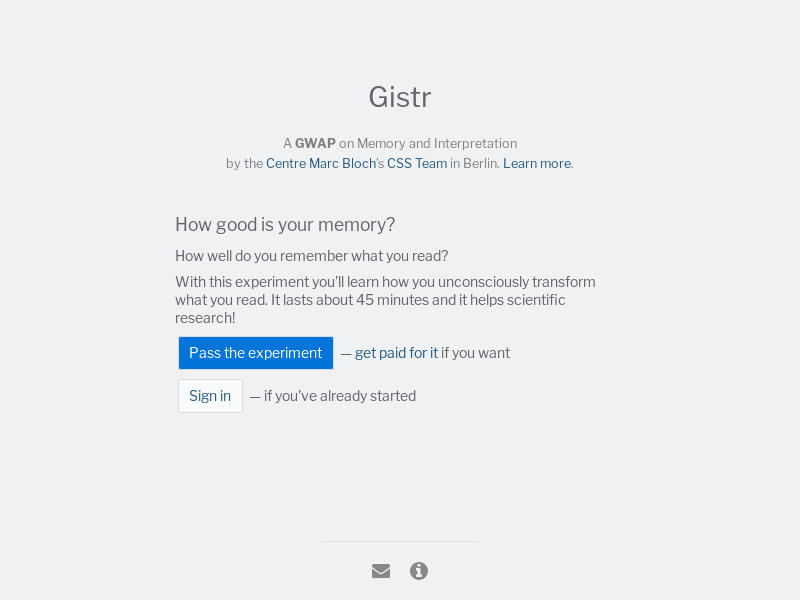
\includegraphics[width=.48\linewidth]{images/manual/gistr-welcome.png}
%%    \label{fig:gistr-welcome}
%%  }
%%  ~
%%  \subfloat[Signup form]{
%%    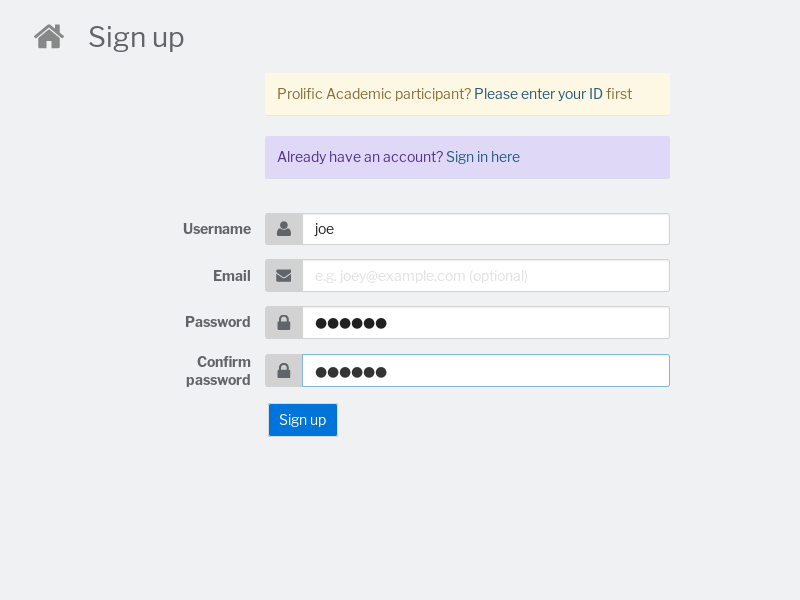
\includegraphics[width=.48\linewidth]{images/manual/gistr-signup.png}
%%    \label{fig:gistr-signup}
%%  }
%%  \caption[Initial steps for a subject entering the experiment]{
%%  \textbf{Initial steps for a subject entering the experiment.}
%%  }
%%  \label{fig:gistr-start}
%%\end{figure}
%%
%%\begin{figure}
%%  \centering
%%  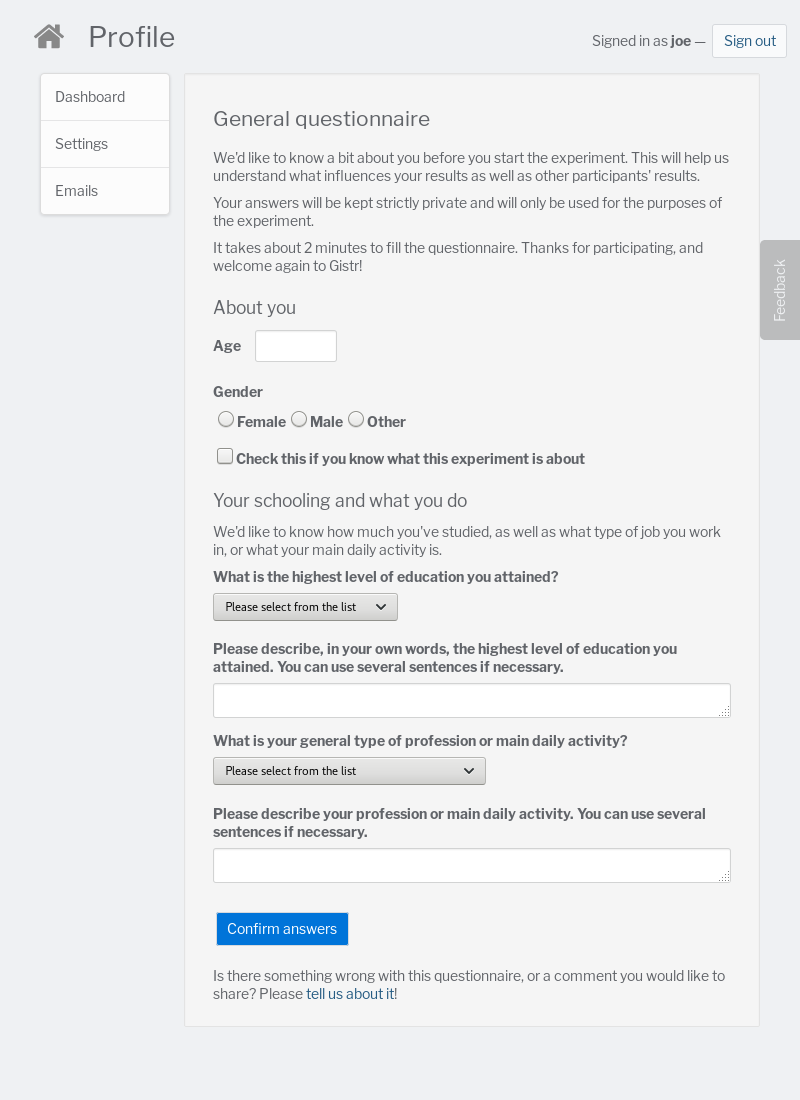
\includegraphics[width=.9\linewidth]{images/manual/gistr-questionnaire.png}
%%  \caption[Initial questionnaire]{
%%  \textbf{Initial questionnaire.}
%%  Subjects can additionally submit feedback on the questionnaire or any other aspect of the experiment on most screens of the website.
%%  }
%%  \label{fig:gistr-questionnaire}
%%\end{figure}

\begin{figure}
  \centering
  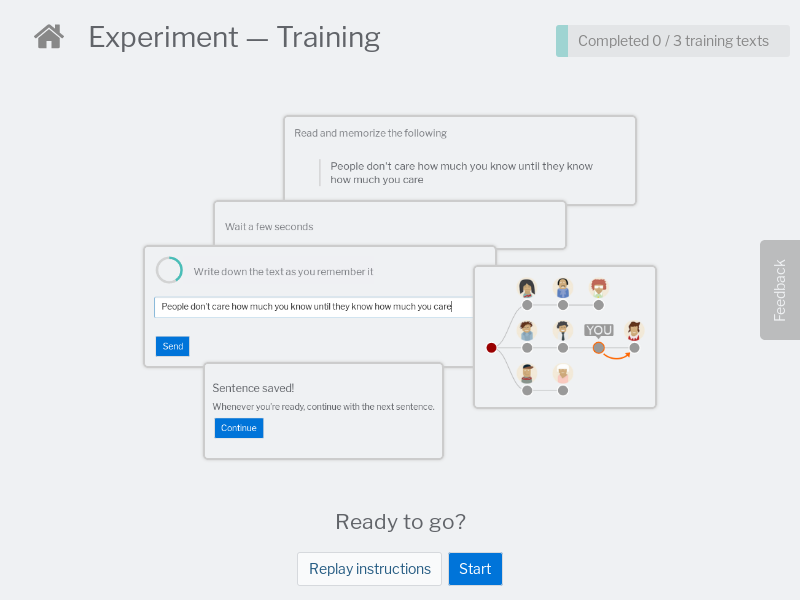
\includegraphics[width=.85\linewidth]{images/manual/gistr-instructions-training.png}
  \caption[Instructions for the main task]{
  \textbf{Instructions for the main task.}
  }
  \label{fig:gistr-instructions}
\end{figure}

\begin{figure}
  \centering
  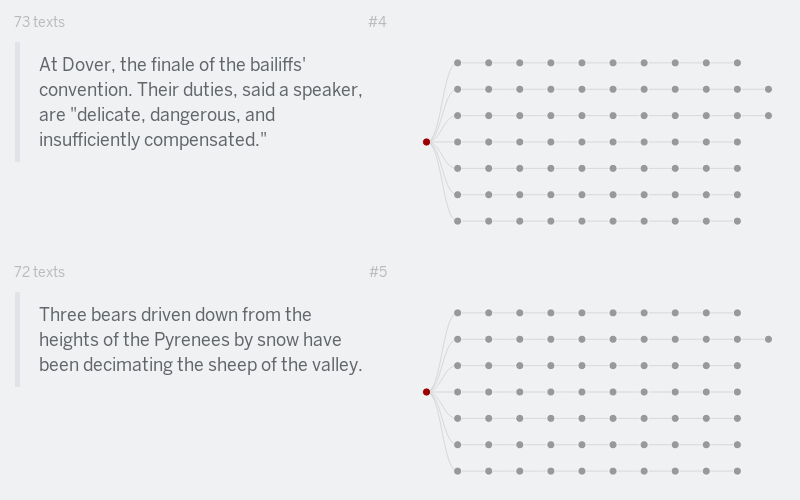
\includegraphics[width=.85\linewidth]{images/manual/gistr-trees.png}
  \caption[Example reformulation trees]{
  \textbf{Example reformulation trees.}
  Two example reformulation trees generated by the setup, targeted at 7 branches of depth 10:
  the text on the left is the initial utterance for all branches of a tree, represented by a red dot in the right-hand graph; each grey dot in the graph represents an utterance produced by a subject on the basis of the preceding dot.
  Subjects create at most one reformulation in each tree, and most create exactly one per tree.
  %The fact that some subjects drop out before completing all their trees leads us to recruit new subjects to fill in the missing reformulations, which is why some branches are uneven.
  }
  \label{fig:gistr-trees}
\end{figure}

Technically, the platform is a complete Web application based on current
technologies, with accompanying backend server to collect and distribute
utterances.
The experiment is available at \url{https://gistr.io} and subject
recruitment was done using Prolific Academic, a service analogous to
Amazon Mechanical Turk and geared towards academic research.

Using the Prolific Academic service allowed us to select among a pool of
over \num{26000} subjects, for which we used the following criteria: (i) first language English speaker, (ii) at least 18 years old, (iii) current country of residence and place of most time spent before
  turning 18 must both be in the UK, (iv) normal or corrected-to-normal vision, (v) no diagnosed literary difficulties, (vi) completed secondary school and (vii) not having participated in any of the preceding experiments.
Only the first two constraints were enforced for the first experiment,
and the full set was used for all subsequent runs. The full filter
provided over \num{2300} eligible subjects, from which the service
automatically sampled the requested number.

Experiment 1 was the first non-trivial launch of the platform, with an
initial 48 subjects, 54 root utterances, and trees targeted for 6
branches of depth 8. Subjects took an average 64 minutes to complete the
experiment, and were rewarded with £6.5. We gathered a total of 2695 utterance reformulations, slightly above the planned \(54 \times 6 \times 8 = 2592\) reformulations due to a minor technical issue.
%%A software bug that appeared
%and had to be fixed halfway through the experiment led the Prolific
%Academic service to recruit more subjects than was originally asked for,
%and the final number of participants was 53,\footnote{The bug appeared
%  only once a large proportion of trees had reached their target depth,
%  and then affected all the subjects nearing completion of the
%  experiment. The time taken to respond to complaints and realise that
%  the experiment had to be paused led some subjects to exceed the
%  maximum allowed time on Prolific Academic, and the service then sent
%  the experiment out to new subjects. After fixing the bug, most
%  subjects who had started the experiment accepted to finish it, leading
%  the final subject count to be higher than originally requested.}
%gathering a total 2695 utterance reformulations (above the planned
%\(54 \times 6 \times 8 = 2592\) reformulations).
Manual inspection
showed that large portions of the data were of poor quality, both
linguistically and because of technical inefficiencies leading to badly
shaped trees; the sections below provide further details on these
questions. Pilots following Experiment 1 were therefore aimed at
improving data quality and solving tree shaping issues. Experiment 2 was
launched with 49 subjects, 50 root utterances, and trees targeted for 7
branches of depth 7, gathering a total 2450 utterance transformations.
Subjects took an average 43 minutes to complete the experiment, and were
rewarded with £6. Quality issues in this data set were solved, but the
choice of source utterances proved too easy to trigger varied
transformations. After pilots exploring different fits of task
parameters with source complexity, Experiment 3 took advantage of a more
complex set of source utterances. It was launched with two batches of 70
subjects each receiving 25 root utterances, and trees targeted for 7
branches of depth 10, gathering a total 3546 utterance transformations.
Subjects took an average 37 minutes to complete the 25 transformations,
and were rewarded with £4.25 on average.

%We now detail the evaluation of data quality and the measures that were
%taken to improve it. The section after that will focus on the fit of
%task parameters and source complexity, before moving on to the analysis
%and results.

\subsection{Data quality}\label{data-quality}

The choice of a Web-based setup sets the requirements of the interface
much higher than for a laboratory experiment. There is no opportunity
for a face-to-face walk-through of the experiment or for questions, and
subtle changes in the way the interface reacts to actions can lead
subjects to interpret a signal where none was intended, or conversely to
not notice an important message.
%%The time of the subjects is not booked,
%%and not having to travel to the laboratory or to talk to someone renders
%%the interaction free of any commitment and generally more consumable:
%%subjects can leave whenever they want, without having to feel bad about
%%it (the only cost being the loss of their reward). The lack of human
%%interaction with the experimenter also removes a natural incentive for
%%subjects to take their time and perform according to what the
%%experimenter in front of them explained. Combined together, these
%%factors mean that if the interface is strenuous or ambiguous in any way,
%%subjects will often pick the interpretations that make the process
%%faster and either complete the experiment with minimal engagement or
%%drop out. Redacting detailed textual instructions often makes matters
%%worse. Instead, t
The interface must lead the subjects through the
necessary explanations while remaining enjoyable, and must be
unambiguous while still hinting towards the expected behaviour at the
right moment, either through subtle interface reactions or through
explicit contextual aids.
%\subsubsection{Manual spam-coding}\label{manual-spam-coding}
Failure to properly encourage and wherever possible enforce the
experiment's expectations led to data riddled with spurious
transformations. Manual inspection of the data collected through
Experiment 1, for which a substantial effort on instructions and for the
overall interface had already been made, showed that large portions of
the data were not usable as such.

We therefore spam-coded utterances for all experiments by hand. An utterance
with any of the following properties was coded as spam:
(i)
  An ellipsis (\enquote{\ldots{}}) or other special characters (e.g.
  \enquote{\textgreater{}}, \enquote{\textless{}}) are present;
(ii)
  The utterance is partly or completely addressed to the experimenter
  (e.g. \enquote{Sorry, I can't remember});
(iii)
  Over half the words are misspelled;
(iv)
  The utterance has no relationship to its parent utterance (i.e.~it is
  an entirely new utterance);
(v)
  The utterance does not stand as an autonomous sentence, either because
  it is truncated or because so many words are garbled it becomes
  nonsense.
\footnote{Note that the last two criteria are not sharp, and several borderline
cases had to be decided for the last one in particular. In Experiment 1
for instance, a subtle misunderstanding allowed by the interface led
subjects to submit some sentences truncated at exactly 10 words, without
regard to their meaning (see the details below); such utterances were
unambiguously incomplete, and were thus coded as spam. In subsequent
experiments however, utterances that could be made complete with the
addition or the deletion of a single, sometimes unimportant word, were
questioned by the same criterion. For instance the simple sentence
\enquote{Mr Jones was robbed during} can be completed by adding the word
\enquote{dinner} at the end, or by removing the word \enquote{during}.
Such sentences do not seem tied to a misunderstanding of the task, and
are arguably attributable to temporary distraction whose effects are
relevant to our analysis. The benefit of the doubt was given to such
utterances, and they were not coded as spam.}
Spam in transmission chains has the additional property of invalidating
all the subsequent utterances, leading to discard more utterances than the ones where subjects introduced spam for the first time.
Coded this way, Experiment 1 showed an accumulated spam rate of 22.4\%.
Combined with an initial technical oversight, where participants could concurrently participate in the same reformulation on the same branch and which led a small portion of
utterances to be misplaced in the chains,
%%\footnote{Ensuring that no two
%%  subjects are creating reformulations for the same chain tip at the
%%  same time, while not blocking other subjects from moving on with the
%%  experiment, is a non-trivial technical hurdle. Not solving it leads
%%  the chains to have \enquote{forks}, that is, utterances with several
%%  children (possibly extending to sub-branches) instead of a single one.
%%  One of the children must then be chosen to form the main chain, and
%%  the others discarded. Solutions to the problem are difficult to test
%%  in practice, as they involve simulating dozens of subjects
%%  concurrently sending utterances to the platform. The approach adopted
%%  in Experiment 1 relied on client-side randomisation, but proved
%%  insufficient: 3.5\% of the utterances posted by subjects were forks
%%  deep in the chains. Experiments 2 and 3 relied on a mix of client-side
%%  randomisation and server-side locking to solve the problem.}
a total of 25.9\% of the utterances generated by Experiment 1 were discarded.
The number of valid transformations garnered by this experiment thus
went from 2695 to 1980. Apart from reducing the size of the usable data,
spam also leads to uneven chains across trees, a heterogeneity that
complicates the analysis. Accepting this level of spam was therefore not
an option.

The main tool we used to reduce the level of spam is the user interface.
As explained above, minor changes in the way the interface reacts to the
subjects' actions combined with relevant context-dependent information
can have a comparatively large impact on spam.
The situation is similar to that of surveys, where much effort is put
into mitigating the risk of users engaging the minimum possible effort
to complete the survey \citep{krosnick_threat_2000}. Successfully
tuning the user interface is therefore a crucial factor in the quality
of the data collected: what the interface might lead subjects to see as
acceptable can easily be spam for the experimenter, and both
perspectives must be aligned as much as possible. Interface design
problems appeared repeatedly throughout the development of the platform
and the pilots. The most important points can be summed up as follows:
(i)
  \emph{Preventing digital copy-paste} (an obvious workaround)
  %: an obvious workaround to the
  %task that most subjects will try in the first few trials.
(ii)
  \emph{Avoiding signals that may be interpreted as a success} (such as avoiding to disable the ``send'' button below a certain number of words, which led some participants to validate their input as they reached the threshold);
%  : a well-known behaviour in transmission
%  chains of linguistic content is the rapid reduction in size of the
%  content that is transmitted
%  \citep{maxwell_remembering_1936,bangerter_transformation_2000,mesoudi_hierarchical_2004}.
%  In order to encourage subjects to rely on what they remember, and
%  prevent them from quickly reaching empty sentences, an early version
%  of the experiment would disable the \enquote{send} button if the
%  subject's input was shorter than 10 words (Experiments 2 and 3 later
%  relaxed this constraint to 5 words). However, some subjects
%  interpreted the button becoming active after 10 words as a signal that
%  their input was ready to be sent as is, even if it was only a partial
%  sentence. This ambiguity, corrected in later versions, is responsible
%  for a large part of the spam found in Experiment 1.
(iii)
  \emph{Improving input quality} (including emphasizing the importance of transmitting correct sentences to the next participants);
%  : Experiment 1 and subsequent pilots
%  showed the need for strong incentives to write well-edited meaningful
%  text. Indeed when pressed for time, some subjects will tend to write
%  misspelled, poorly punctuated, or even meaningless utterances, which
%  invalidate all the sentences that follow in the branch. Countering
%  this tendency involved several changes to Experiments 2 and 3:
%  emphasis was added to the fact that what is produced by one subject is
%  later sent to other subjects, encouraging a more conscientious
%  behaviour; a bonus was associated with high-fidelity trials, and the
%  top 5 subjects with lowest transformation rates (as defined below in
%  the analysis) received increased payment; most importantly, input from
%  the subjects was also checked for repeated or inadequate punctuation,
%  and for correct spelling against a combined British and American
%  English dictionary. The interface asked subjects to correct any input
%  that failed those tests, and presented them with a short explanation
%  that emphasised the faulty behaviour and recalled the chain structure
%  of the experiment. Inspecting the platform logs showed that this last
%  measure led subjects to often correct their utterances, a fact that
%  was also confirmed by the increased average writing time.
(iv)
  \emph{Relaxing the time pressure} (and avoiding rushed behaviors, by enforcing a minimal reading time);
%%  : the interface of Experiment 1 made
%%  several mistakes that worsened the inherent pressure on subjects to
%%  complete the study as fast as possible (indeed, payment on Prolific
%%  Academic is per experiment, not per time spent -- which, conversely,
%%  would encourage subjects to be very slow). First, subjects could
%%  terminate the reading time of an utterance at will. While this
%%  provided a measure of the effective reading time used by subjects, it
%%  also opened the possibility of speeding through the trials. Indeed
%%  over a third of the transformations of Experiment 1 were done by using
%%  less than half the allotted reading time. This pressure was increased
%%  by the presence of a \enquote{remaining time} clock in the reading and
%%  waiting phases, similar to the green clock shown on
%%  \cref{fig:gistr-instructions} for the writing phase. By removing
%%  superfluous clocks, keeping the reading time fixed, and proposing a
%%  break after each utterance, Experiments 2 and 3 relaxed the time
%%  pressure on the subjects and improved the final data quality.
(v)
  \emph{Feedback channel} (for subjects to comment on the
  questions they were asked); and
%%  , and encourage the use of debriefing
%%  sessions to deepen that understanding
%%  \citep{de_leeuw_international_2008}. Such feedback channels have
%%  also become a norm in online services, and we therefore chose to give
%%  the possibility for subjects to comment on most screens of the
%%  experiment (excluding the read-write screens) through a side-ribbon
%%  which, when clicked, would overlay a comment box (see
%%  \cref{fig:gistr-feedback}). It seems, however, that a more interactive
%%  option would be more effective, as only a handful of subjects entered
%%  comments over the course of Experiments 2 and 3.
(vi)  \emph{Instructions} (fine-tuning the exact phrasing of instructions and making it more ergonomic).
%% of the   making the
%%  interface for instructions palatable using a now common pattern: for
%%  the instructions pictured in \cref{fig:gistr-instructions} for
%%  instance, different elements or images are successively foregrounded
%%  and highlighted, and a tooltip with short explanations appears next to
%%  the active element.\footnote{The pattern was popularised by software
%%    libraries such as Intro.js (\url{http://introjs.com/}).} Here too,
%%  Experiment 1 and subsequent pilots allowed users to skip these
%%  instructions, leading a portion of the subjects to effectively never
%%  read them. Experiments 2 and 3 made navigating the complete list of
%%  instructions mandatory in order to start the trials.
%%\end{itemize}

These changes reduced the spam rate drastically. On the same criteria as
Experiment 1, Experiment 2 showed an accumulated spam rate of .8\%,
which combined with misplaced utterances led to a total 1.4\% of
utterances discarded (leading to a final 2411 valid transformations).
Experiment 3 showed an accumulated spam rate of 1.0\%, and with
misplaced utterances had to discard a total 1.1\% of the data (leading
to a final 3506 valid transformations).

%\begin{figure}
%  \centering
%  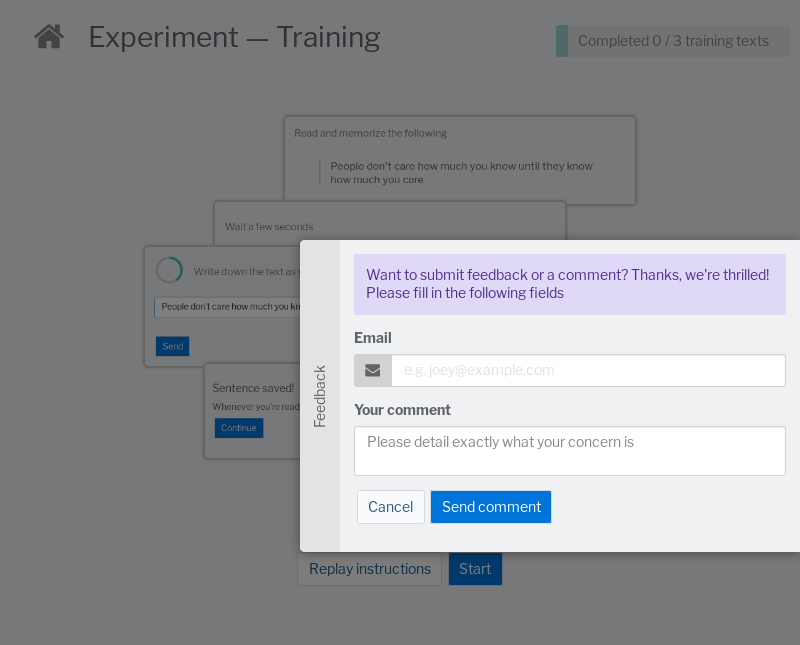
\includegraphics[width=.75\linewidth]{images/manual/gistr-feedback.png}
%  \caption[Overlay feedback box]{
%  \textbf{Overlay feedback box.}
%  Opened in the instructions screen from Fig.~\ref{fig:gistr-instructions}.
%  The box is available in most screens of Experiments 2 and 3.
%  }
%  \label{fig:gistr-feedback}
%\end{figure}
%
\subsection{Task difficulty and source complexity
fit}\label{task-difficulty-and-source-complexity-fit}

In the simple task we used, difficulty is controlled by the reading time
allotted to subjects and by the selection of source utterances. To unify reading times
 across utterances we made them proportional to the number of words \(|u|_w\) in a given utterance \(u\):
reading time is defined as \(|u|_w \cdot r\), with \(r\) the
\emph{reading factor}. Average reading speeds for university students
are usually between 200 and 300 words per minute, that is between 3.33
and 5 words per second \citep%[see][where fast readers average at 330~wpm and slow readers average at 207~wpm]
{rayner_eye_2010}. A reading factor of \(r = 1\) therefore gives fast readers the time to read
utterances more than 5 times, and slow readers about 3 to 4 times. A
reading factor of \(r = .3\) gives fast readers one or two readings, and
slow readers at least one. \(r = .2\) gives some readers one reading and
others less than one, and \(r = .1\) lets readers simply glance at the
utterances without being able to read them completely.

Pilots and manual exploration indicated that the difficulty of the task
is not linear with \(r\). Whatever the value of \(r\), longer utterances
(more than 25 words) are often more transformed, relative to their
length, than shorter utterances; longer utterances also give more space
for the subjects to reformulate, leading to more changes in style and
permutations in the words. Changing \(r\) has less effect on shorter
utterances than on longer utterances, and on utterances in oral versus
written style. For short utterances in an oral style, pilots indicated
that there is an abrupt transition between a low transformation regime
when subjects can read the sentence at least once, and an extremely
noisy regime when the subjects do not have the time to read the
utterances entirely at their normal speed. Conversely, the transition is
smoother for longer utterances or utterances with a more formal written
style. Choosing an adequate set of source utterances is therefore an
integral factor in adjusting the difficulty of the task.

Changing the source utterances also affects the sampling bias in ways
that are difficult to measure given the multidimensionality of text.
Contrasting minimally different utterances in different domains has
resulted in domain-specific outcomes on for instance stereotypes,
information hierarchy, and counter-intuitiveness
\citep{kashima_maintaining_2000,mesoudi_bias_2006,barrett_spreading_2001,mesoudi_multiple_2008},
and authors have suggested that these outcomes are related to
domain-specific biases in transformations (although to our knowledge
these effects have not yet been studied jointly). In spite of this, we
hypothesise that the low-level cognitive mechanisms underlying utterance
transformation, that is the mechanisms that give rise to such
accumulated outcomes, do not fundamentally change because of the type or
the style of an utterance. If using news quotes instead of movie quotes
or stories is likely to affect parameters of the observed
transformations, it is less likely to affect the structure of the
underlying cognitive mechanism, and therefore the general structure of
transformations. Making this hypothesis lets us use utterance selection
as an exploratory tool: by altering both the sampling of the
transformations and the task difficulty, the exploration of different
styles and types can help (1) improve data quality and (2) make the
general structure more visible, thus easier to measure and characterise.
%%\footnote{If this exploration yields insights about the structure of
%%transformations and their effects in the long term, and if such insights
%%are consistent with the previous chapter, then it will make sense to ask
%%to what extent the uncovered structure is applicable to or varies with
%%other types of utterances. Throughout pilots and experiments, our goal
%%was therefore to find a set of utterances which would trigger varied
%%transformations whose structure we could analyse, while at the same time
%%helping the subjects to produce quality data by not creating too much
%%pressure with reading time.}

The set of sources used in Experiment 1 covered a broad spectrum of
utterance types sampled from the following categories:

\begin{itemize}
\item
  Quotes found in blog posts from the MemeTracker data set \citep{leskovec_meme-tracking_2009} and used in a recent article on sentence reformulation \citep{lerique-2018-semantic-drift},
\item
  Famous compelling quotes from Wikisource\footnote{\url{https://en.wikisource.org/}.}
  such as \enquote{Never doubt that a small group of thoughtful
  committed citizens can change the world, it is the only thing that
  ever has},
\item
  Quotes extracted from the movie \emph{12 Angry Men} such as
  \enquote{If you ask me I'd slap those tough kids down before they
  start any trouble, it saves a lot of time and money},
\item
  Excerpts from news stories on controversial subjects (such as
  \enquote{How will the cultural and religious aspects of so many
  migrants impact E.U. society?}) or risk-related subjects such as
  stories about the risks of Triclosan \citep%[used by][ in their  study of the amplification of risk perception]
{moussaid_amplification_2015},
\item
  The tale \enquote{War of the Ghosts} used by
  \citet{bartlett_remembering:_1995} in his original
  studies,\footnote{Available online at
    \url{http://penta.ufrgs.br/edu/telelab/2/war-of-t.htm}.} as well as
  excerpts from other tales,
\item
  A small number of hand-crafted sentences such as surprising statements
  (\hbox{e.g.} \enquote{Don't forget to leave the door open when you leave the
  office}) or stereotype-incongruent statements (\hbox{e.g.} \enquote{The young
  boy was suddenly hit by the little girl}).
\end{itemize}

Each of these categories, we thought, could encourage the triggering of
transformations. The spam level of Experiment 1, and especially the
amount of misspelled words, made the exploration of the detailed
transformations impossible and shifted the focus towards improving data
quality through the interface. Nonetheless, it became clear that using
such a heterogeneous set of utterances could surprise subjects, and was
not the best approach to elicit regularities in transformations.
Experiments 2 and 3 relied on a more thorough exploration of possible
source data sets. Pilots explored utterances extracted from previous
studies \citetext{\citealp{bangerter_transformation_2000} on personification and increased
stereotypes, \citealp{heath_emotional_2001} on the role of disgust, \citealp{maxwell_remembering_1936} on incoherent stories, \citealp{mesoudi_bias_2006} for the role of social information}.

Two larger and more homogeneous sets of utterances were reconstituted
and finally used in Experiments 2 and 3. First, a set of movie quotes
provided by \citet{danescu-niculescu-mizil_you_2012}. This data set
contains about 2200 pairs of quotes extracted from 1000 movie scripts;
each pair is made of a quote that was marked as memorable by users of
the Internet Movie Database, coupled with the closest quote in the same
movie script that is spoken by the same character, has the same number
of words, but is not marked as memorable on the Internet Movie Database.
The 2200 pairs of quotes were filtered to keep only those which passed
the spelling and punctuation quality tests from the previous section,
and for which the number of words was strictly matched when excluding
punctuation (this left 505 pairs). Here is an example pair from this
data set (first the memorable quote, then the non-memorable
counterpart):

\begin{quote}
\enquote{The first and most important rule of gunrunning is never get
shot with your own merchandise.}
\end{quote}

\begin{quote}
\enquote{At least when they say they're going to have a war, they keep
their word.}
\end{quote}

Second, a set of short stories from \citet{feneon_novels_2007} was
used. These stories are productions from Félix Fénéon originally
anonymously published in the French newspaper \emph{Le Matin} in 1906.
They describe facts from everyday life such as accidents, suicides, or
trials, in a terse and sometimes humorous style. The following example
illustrates the style of these stories:

\begin{quote}
\enquote{An unidentified maker of paste jewels from the third district
was fishing in a boat with his wife at Maldon. She fell. He dived. Both
gone.}
\end{quote}

A sample of 60 stories was extracted from the English version, for which
French names and places were replaced with names and places more
familiar to British subjects. Pilots explored these sets of utterances
with reading factors of .1, .2, .3, .75 and 1. Finally, tests were also
made using these utterances with content words replaced with
pseudo-words, in order to restrict effects to the grammatical dimension
only.\footnote{Pseudo-words were generated using the Wuggy library
  \citep{keuleers_wuggy:_2010}.} The pseudo-word tests turned out not
to fit our exploration framework however, as the task became too
confusing and subjects often replaced unknown words with real words.

Experiment 2 used 25 of the 27 pairs of movie quotes that had exactly 15
or 16 words, providing a homogeneous set of 50 utterances in oral style,
with a reading factor of .75. Experiment 3 used 43 of the 60 short
stories by Fénéon (average number of words \num{21.2}) coupled with 4
utterances extracted from \citet{mesoudi_bias_2006} (average number
of words \num{60.3}) and 3 utterances extracted from the story used by
\citet{maxwell_remembering_1936} (average number of words
\num{40.7}), with a reading factor of 1.







%%%%%%%%%%%%%%%%%%%%%%%%%%%%%%%%%%%%%%%%%%%%%%%%%%%%%%%%%%%%%%%%%%%%%%%%%%%
%%%%%%%%%%%%%%%%%%%%%%%%%%%%%%%%%%%%%%%%%%%%%%%%%%%%%%%%%%%%%%%%%%%%%%%%%%%
%%%%%%%%%%%%%%%%%%%%%%%%%%%%%%%%%%%%%%%%%%%%%%%%%%%%%%%%%%%%%%%%%%%%%%%%%%%
%%%%%%%%%%%%%%%%%%%%%%%%%%%%%%%%%%%%%%%%%%%%%%%%%%%%%%%%%%%%%%%%%%%%%%%%%%%
%%%%%%%%%%%%%%%%%%%%%%%%%%%%%%%%%%%%%%%%%%%%%%%%%%%%%%%%%%%%%%%%%%%%%%%%%%%
%%%%%%%%%%%%%%%%%%%%%%%%%%%%%%%%%%%%%%%%%%%%%%%%%%%%%%%%%%%%%%%%%%%%%%%%%%%
%%%%%%%%%%%%%%%%%%%%%%%%%%%%%%%%%%%%%%%%%%%%%%%%%%%%%%%%%%%%%%%%%%%%%%%%%%%
%%%%%%%%%%%%%%%%%%%%%%%%%%%%%%%%%%%%%%%%%%%%%%%%%%%%%%%%%%%%%%%%%%%%%%%%%%%
%%%%%%%%%%%%%%%%%%%%%%%%%%%%%%%%%%%%%%%%%%%%%%%%%%%%%%%%%%%%%%%%%%%%%%%%%%%
%%%%%%%%%%%%%%%%%%%%%%%%%%%%%%%%%%%%%%%%%%%%%%%%%%%%%%%%%%%%%%%%%%%%%%%%%%%
%%%%%%%%%%%%%%%%%%%%%%%%%%%%%%%%%%%%%%%%%%%%%%%%%%%%%%%%%%%%%%%%%%%%%%%%%%%
%%%%%%%%%%%%%%%%%%%%%%%%%%%%%%%%%%%%%%%%%%%%%%%%%%%%%%%%%%%%%%%%%%%%%%%%%%%
%%%%%%%%%%%%%%%%%%%%%%%%%%%%%%%%%%%%%%%%%%%%%%%%%%%%%%%%%%%%%%%%%%%%%%%%%%%
%%%%%%%%%%%%%%%%%%%%%%%%%%%%%%%%%%%%%%%%%%%%%%%%%%%%%%%%%%%%%%%%%%%%%%%%%%%
%%%%%%%%%%%%%%%%%%%%%%%%%%%%%%%%%%%%%%%%%%%%%%%%%%%%%%%%%%%%%%%%%%%%%%%%%%%
%%%%%%%%%%%%%%%%%%%%%%%%%%%%%%%%%%%%%%%%%%%%%%%%%%%%%%%%%%%%%%%%%%%%%%%%%%%


%%%%%%%%    %%%%%%%%    %%%%%%%%    GARBAGE    %%%%%%%%    %%%%%%%%    %%%%


%%%%%%%%%%%%%%%%%%%%%%%%%%%%%%%%%%%%%%%%%%%%%%%%%%%%%%%%%%%%%%%%%%%%%%%%%%%
%%%%%%%%%%%%%%%%%%%%%%%%%%%%%%%%%%%%%%%%%%%%%%%%%%%%%%%%%%%%%%%%%%%%%%%%%%%
%%%%%%%%%%%%%%%%%%%%%%%%%%%%%%%%%%%%%%%%%%%%%%%%%%%%%%%%%%%%%%%%%%%%%%%%%%%
%%%%%%%%%%%%%%%%%%%%%%%%%%%%%%%%%%%%%%%%%%%%%%%%%%%%%%%%%%%%%%%%%%%%%%%%%%%
%%%%%%%%%%%%%%%%%%%%%%%%%%%%%%%%%%%%%%%%%%%%%%%%%%%%%%%%%%%%%%%%%%%%%%%%%%%
%%%%%%%%%%%%%%%%%%%%%%%%%%%%%%%%%%%%%%%%%%%%%%%%%%%%%%%%%%%%%%%%%%%%%%%%%%%
%%%%%%%%%%%%%%%%%%%%%%%%%%%%%%%%%%%%%%%%%%%%%%%%%%%%%%%%%%%%%%%%%%%%%%%%%%%
%%%%%%%%%%%%%%%%%%%%%%%%%%%%%%%%%%%%%%%%%%%%%%%%%%%%%%%%%%%%%%%%%%%%%%%%%%%
%%%%%%%%%%%%%%%%%%%%%%%%%%%%%%%%%%%%%%%%%%%%%%%%%%%%%%%%%%%%%%%%%%%%%%%%%%%
%%%%%%%%%%%%%%%%%%%%%%%%%%%%%%%%%%%%%%%%%%%%%%%%%%%%%%%%%%%%%%%%%%%%%%%%%%%
%%%%%%%%%%%%%%%%%%%%%%%%%%%%%%%%%%%%%%%%%%%%%%%%%%%%%%%%%%%%%%%%%%%%%%%%%%%
%%%%%%%%%%%%%%%%%%%%%%%%%%%%%%%%%%%%%%%%%%%%%%%%%%%%%%%%%%%%%%%%%%%%%%%%%%%
%%%%%%%%%%%%%%%%%%%%%%%%%%%%%%%%%%%%%%%%%%%%%%%%%%%%%%%%%%%%%%%%%%%%%%%%%%%
%%%%%%%%%%%%%%%%%%%%%%%%%%%%%%%%%%%%%%%%%%%%%%%%%%%%%%%%%%%%%%%%%%%%%%%%%%%
%%%%%%%%%%%%%%%%%%%%%%%%%%%%%%%%%%%%%%%%%%%%%%%%%%%%%%%%%%%%%%%%%%%%%%%%%%%
%%%%%%%%%%%%%%%%%%%%%%%%%%%%%%%%%%%%%%%%%%%%%%%%%%%%%%%%%%%%%%%%%%%%%%%%%%%


%%\footnote{The
%%  following three approaches could be combined to counter ordering bias.
%%  (1) Have each subject do a single trial, that is, use as many subjects
%%  as there are reformulations in the full experiment; this is extremely
%%  expensive as there is a fixed minimal price for each subject,
%%  corresponding to the time needed to explore the interface, answer the
%%  initial questionnaire, and train for the main task. (2) Have each
%%  subject wait an adjustable amount of time between each trial, to open
%%  the possibility for ordering subjects differently than their time of
%%  arrival; this is also expensive, as it means paying subjects for
%%  waiting most of the time they spend on the experiment. (3) Optimise
%%  the order of tree presentations of each subject so as to spread
%%  subjects across depths; while this approach could achieve some level
%%  of spread when combined with (2), it is contingent on the starting
%%  times of subjects and their synchronisation, which we do not control
%%  (subjects find the experiment through Prolific Academic notifications
%%  and are free to start whenever they want).}


%  \footnote{The frontend first used the Ember.js framework
%  \citep{ember.js_contributors_ember.js:_2017}, and was later
%  rewritten and extended using the Elm programming language
%  \citep{czaplicki_elm:_2017}. Indeed, the assurance of no runtime
%  exceptions that Elm provides was a strong argument in favour of
%  switching, as was made clear by the trying \enquote{customer support}
%  experience of a bug hitting 40 to 50 subjects at once during
%  Experiment 1. The backend is a Python application written on top of
%  the Django REST framework \citep{christie_django_2017}. Most of the
%  critical logic in the software is verified using automated tests, and
%  the full source code is available under a Free Software licence at
%  \url{https://github.com/interpretation-experiment/gistr-app}
%  (frontend), and
%  \url{https://github.com/interpretation-experiment/spreadr} (backend).}

%%\footnote{The
%%  public url of the experiment was not advertised anywhere else, and
%%  checking the subjects' Prolific Academic ID confirmed that only people
%%  from that platform participated in each experiment.}


%% -----------------------------------------------------------------------------------------------------------------------------------------


\printcredits

\section*{Acknowledgements}
\rk{todo}

\section*{Software colophon}
\rk{todo}

%% Loading bibliography style file
\bibliographystyle{cas-model2-names}

% Loading bibliography database
\bibliography{gistr}

\end{document}
